\documentclass{beamer}

\useoutertheme[subsection=false]{miniframes}
\usecolortheme{beaver}
\setbeamertemplate{navigation symbols}{}
\setbeamertemplate{footline}{}
\usepackage{graphicx}
\usepackage{url}
\usepackage{datetime}
\usepackage{tikz-cd}
\newcommand{\lectureDate}{\formatdate{06}{11}{2018}}

\setbeamertemplate{caption}
{\raggedright\insertcaption\par}
\title{MATH211: Linear Methods I}
\author{Matthew Burke}
\date{\lectureDate}
\begin{document}

\frame{\titlepage}

\begin{frame}{Lecture on \lectureDate}
  \tableofcontents
\end{frame}

\section*{Last time}
\label{sec:Last-time}

\begin{frame}{Last time}
  \begin{itemize}
  \item Matrices and linear transformations\vfill
  \item Composition of linear transformations\vfill
  \item Inverse of linear transformations
  \end{itemize}
\end{frame}

\section{Examples}

\begin{frame}
\begin{beamercolorbox}[sep=12pt,center]{part title}
\usebeamerfont{section title}
\insertsection\par
\end{beamercolorbox}
\end{frame}

\begin{frame}{Examples}
\begin{example}
If
\begin{equation*}
S \left[
\begin{array}{c}
x\\
y
\end{array}
\right] = \left[
\begin{array}{c}
x\\
-y
\end{array}
\right]\text{ and } T \left[
\begin{array}{c}
x\\
y
\end{array}
\right] = \left[
\begin{array}{c}
-y\\
x
\end{array}
\right]
\end{equation*}
then find $S\circ T$, $T\circ S$ and the matrices $[S\circ T]$ and $[T\circ S]$.
\end{example}

\begin{example}
If
\begin{equation*}
T \left[
\begin{array}{c}
x\\
y
\end{array}
\right] = \left[
\begin{array}{c}
x+y\\
y
\end{array}
\right]
\end{equation*}
find $T^{-1}$ and $[T^{-1}]$.
\end{example}
\end{frame}


\section{Complex numbers}

\begin{frame}
\begin{beamercolorbox}[sep=12pt,center]{part title}
\usebeamerfont{section title}
\insertsection\par
\end{beamercolorbox}
\end{frame}

\begin{frame}{Progression of thought about complex numbers}

% \begin{quote}
% .. subtle as they are useless ..
% \end{quote}
% (Girolamo Cardano - discoverer of complex numbers)
% \vfill
\begin{quote}
\dots the whole matter seems to rest on sophistry rather than truth\dots
\end{quote}
(Rafael Bombelli 1526-1572. Early innovator in use of complex numbers)
\vfill
\begin{quote}
The shortest path between two truths in the real domain passes through the complex domain.
\end{quote}
(Jacques Hadamard 1865-1963)
% \begin{quote}
% Indeed, nowadays no electrical engineer could get along without complex numbers, and neither could anyone working in aerodynamics or fluid dynamics.
% \end{quote}
% (Keith Devlin - British mathematician)

% \vfill

% \begin{quote}
% The imaginary number is a fine and wonderful resource of the human spirit, almost an amphibian between being and not being.
% \end{quote}
% (Leibniz)
\end{frame}

% \begin{frame}{More recently...}
% \begin{quote}
% It has been written that the shortest and best way between two truths of the real domain often passes through the imaginary one.
% \end{quote}
% (Jacques Hadamard)
% \vfill

% \begin{quote}
% I tell you, with complex numbers you can do anything.
% \end{quote}
% (John Derbyshire - mathematics writer)
% \vfill

% \begin{quote}
% Indeed, nowadays no electrical engineer could get along without complex numbers, and neither could anyone working in aerodynamics or fluid dynamics.
% \end{quote}
% (Keith Devlin - British mathematician)
% \end{frame}

\begin{frame}{Algebraic motivation - extending the number system}
Suppose that we only knew about the natural numbers:
\begin{equation*}
\mathbb{N} := \{0, 1, 2, 3, \dots\}.
\end{equation*}
Then we wouldn't have a solution to the equation:
\begin{equation*}
 x + 1 = 0
\end{equation*}
{\bf Solution:}
\begin{itemize}
	\item Add a new symbol $-1$ such that
	\begin{equation*}
	(-1)+1 = 0
	\end{equation*}
	\item Figure out addition and multiplication for this new symbol.
	\item (So in particular forced to add $-k$ for all $k\in \mathbb{N}$.)
\end{itemize}
\end{frame}

\begin{frame}{Algebraic motivation - extending the number system}
\begin{quote}
God made the integers; all else is the work of man.
\end{quote}
(Leopold Kronecker 1823-1891)\vfill
\begin{itemize}
	\item Using only positive integers $\{1, 2, 3, \dots\}$
	\begin{itemize}
		\item we cannot find a solution to $x+1 = 0$.
	\end{itemize}\vfill
	\item Using only integers $\{\dots, -2, -1, 0, 1, 2, \dots\}$
	\begin{itemize}
		\item we cannot find a solution to $3x+2 = 0$.
	\end{itemize}\vfill
	\item Using only fractions $\{\frac{a}{b} \text{ where } b\neq0 \}$
	\begin{itemize}
		\item we cannot find a solution to $x^2-2 =0$.
	\end{itemize}\vfill
	\item Using only real numbers (decimals)
	\begin{itemize}
		\item we cannot find a solution to $x^2 + 1 = 0$\dots
	\end{itemize}
\end{itemize}
\end{frame}

\begin{frame}{Algebraic motivation - extending the number system}
Suppose that we only knew about real numbers.\vfill
Then we wouldn't have a solution to the equation:
\begin{equation*}
 x^2 + 1 = 0
\end{equation*}
{\bf Solution:}
\begin{itemize}
	\item Add a new symbol $i$ such that
	\begin{equation*}
	i^2 = -1
	\end{equation*}
	\item Figure out addition and multiplication for this new symbol.
	\begin{itemize}
		\item (Later in this lecture.)
	\end{itemize}
	\item It turns out that we are forced to add all numbers of the form:
	\begin{equation*}
	a+ib
	\end{equation*}
	where $a$ and $b$ are real numbers.
\end{itemize}
\end{frame}

\begin{frame}{Complex numbers}
\begin{definition}
\begin{itemize}
\item
The \emph{imaginary unit}, denoted $i$, is defined to be
a number with the property that $i^2=-1$.
\item
A \emph{pure imaginary} number has the form $bi$ where 
$b\in \mathbb{R}$, $b\neq 0$.
\item
A \emph{complex number} is any number $z$ of the form
\[ z = a + bi\]
where $a,b\in \mathbb{R}$ and $i$ is the imaginary unit.
\end{itemize}
\end{definition}
\begin{definition}
If $z = a + bi$ then:
\begin{itemize}
\item
$a$ is called the \emph{real part} of $z$.
\item
$b$ is called the \emph{imaginary part} of $z$.
\end{itemize}
\end{definition}
\end{frame}

\begin{frame}{Questions}
Questions?
\end{frame}

\section{Plus and times}

\begin{frame}
\begin{beamercolorbox}[sep=12pt,center]{part title}
\usebeamerfont{section title}
\insertsection\par
\end{beamercolorbox}
\end{frame}

\begin{frame}{Motivation}
Treat $i$ as a number that satisfies the usual laws. E.g.:-
\begin{itemize}
	\item $a(b+c) = ab+ac$
	\item $a+b = b+a$
	\item $ab = ba$ \dots etc \dots
\end{itemize}
as well as
\begin{equation*}
i^2=-1
\end{equation*}
and see what happens.
\begin{example}
\begin{align*}
1+i+i^2+i^3+i^4+i^5 &= 1+i-1-i+1+i \\
&= 1+i
\end{align*}
which cannot be simplified any further.\\
(Because we only know $i^2=-1$.)
\end{example}
\end{frame}

\begin{frame}{Addition}
\begin{example}
We would want addition to satisfy:-
\begin{itemize}
	\item $i+i = 2i$
	\item $i-i = 0$
	\item $(1+i)+2 = 3+i$
\end{itemize}
\end{example}
\begin{definition}
If $a$, $b$, $c$ and $d$ are real numbers then:
	\begin{equation*}
	(a+bi)+(c+di) = (a+c)+(b+d)i
	\end{equation*}
\end{definition}
\end{frame}

\begin{frame}{Multiplication}
\begin{example}
We would want multiplication to satisfy:-
	\begin{itemize}
		\item $i\cdot i = -1$
		\item $2\cdot i = 2i$
		\item $(1+i)\cdot i = i+i\cdot i = -1+i$
	\end{itemize}
\end{example}
\begin{definition}
If $a$, $b$, $c$ and $d$ are real numbers then
\begin{equation*}
(a+bi)\cdot(c+di) = ac+adi+bci-db = (ac-bd)+(ad+bc)i
\end{equation*}
\end{definition}
\end{frame}


\begin{frame}{Equations}
\begin{definition}
If $a$, $b$, $c$ and $d$ are real numbers then
\begin{equation*}
a+bi = c+di
\end{equation*}
if and only if $a=c$ and $b=d$.
\end{definition}
\end{frame}


\begin{frame}{Questions?}
Questions?
\end{frame}

\begin{frame}{Examples}
\begin{example}
Evaluate
\begin{itemize}
\item $(-3+6i) + (5-i)$.
% Ans: 2+5i
\item $(4-7i) + (6-2i)$.
% 10-9i
\item $(-3+6i) - (5-i)$.
%-8+7i
\item $(4-7i) - (6-2i)$.
%-2-5i
\end{itemize}
\end{example}
\begin{example}
\begin{equation*} 
(2-3i)(-3+4i) 
\end{equation*}
% ANS: 6+17i
\end{example}
\begin{example}
Find all complex numbers $z$ such that $z^2 = -3+4i$.
%% Ans: z = 1+2i or z = -1-2i
\end{example}
\end{frame}

\begin{frame}{Clearing denominators}
\begin{example}[Exemplar]
Write 
\begin{equation*}
\frac{a+bi}{c+di}
\end{equation*}
in the form $e+fi$ for real numbers $a$, $b$, $c$, $d$, $e$, and $f$.
\end{example}
\begin{itemize}
\item $\frac{1}{i}$ % ANS -i
\item $\frac{2-i}{3+4i}$ % ANS 2/25 -(11/25)i
\item $\frac{1-2i}{-2+5i}$ % ANS -(12/29) -(1/29)i
\end{itemize}
\end{frame}

\section{Graphical interpretation}

\begin{frame}
\begin{beamercolorbox}[sep=12pt,center]{part title}
\usebeamerfont{section title}
\insertsection\par
\end{beamercolorbox}
\end{frame}

\begin{frame}[fragile]{Graphical interpretation}
Consider the function $\mathbb{R} \rightarrow \mathbb{R}$ that multiplies by $-1$:
\begin{equation*}
\begin{tikzcd}
-3\arrow[bend left, color = blue]{rrrrrr} & -2\arrow[bend left, color = blue]{rrrr} & -1 \arrow[bend left, color = blue]{rr} & 0 & +1\arrow[bend left, color = blue]{ll} & +2\arrow[bend left, color = blue]{llll} & +3\arrow[bend left, color = blue]{llllll}\\
\end{tikzcd}
\end{equation*}
which shows us that $-1\times(-1\times x) = x$.
\end{frame}

\begin{frame}[fragile]{Graphical interpretation}
So how do we get a transformation that squares to $-1$?
\begin{equation*}
\begin{tikzcd}
{} & {} & +i \arrow[bend right, color = blue]{dl} & {} & {}\\
-2 & -1\arrow[bend right, color = blue]{dr} & 0 & +1 \arrow[bend right, color = blue]{ul} & +2\\
{} & {} & -i\arrow[bend right, color = blue]{ur} & {} & {}
\end{tikzcd}
\end{equation*}
\end{frame}

\begin{frame}[fragile]{Graphical interpretation}
\begin{columns}
	\column{0.5\textwidth}
	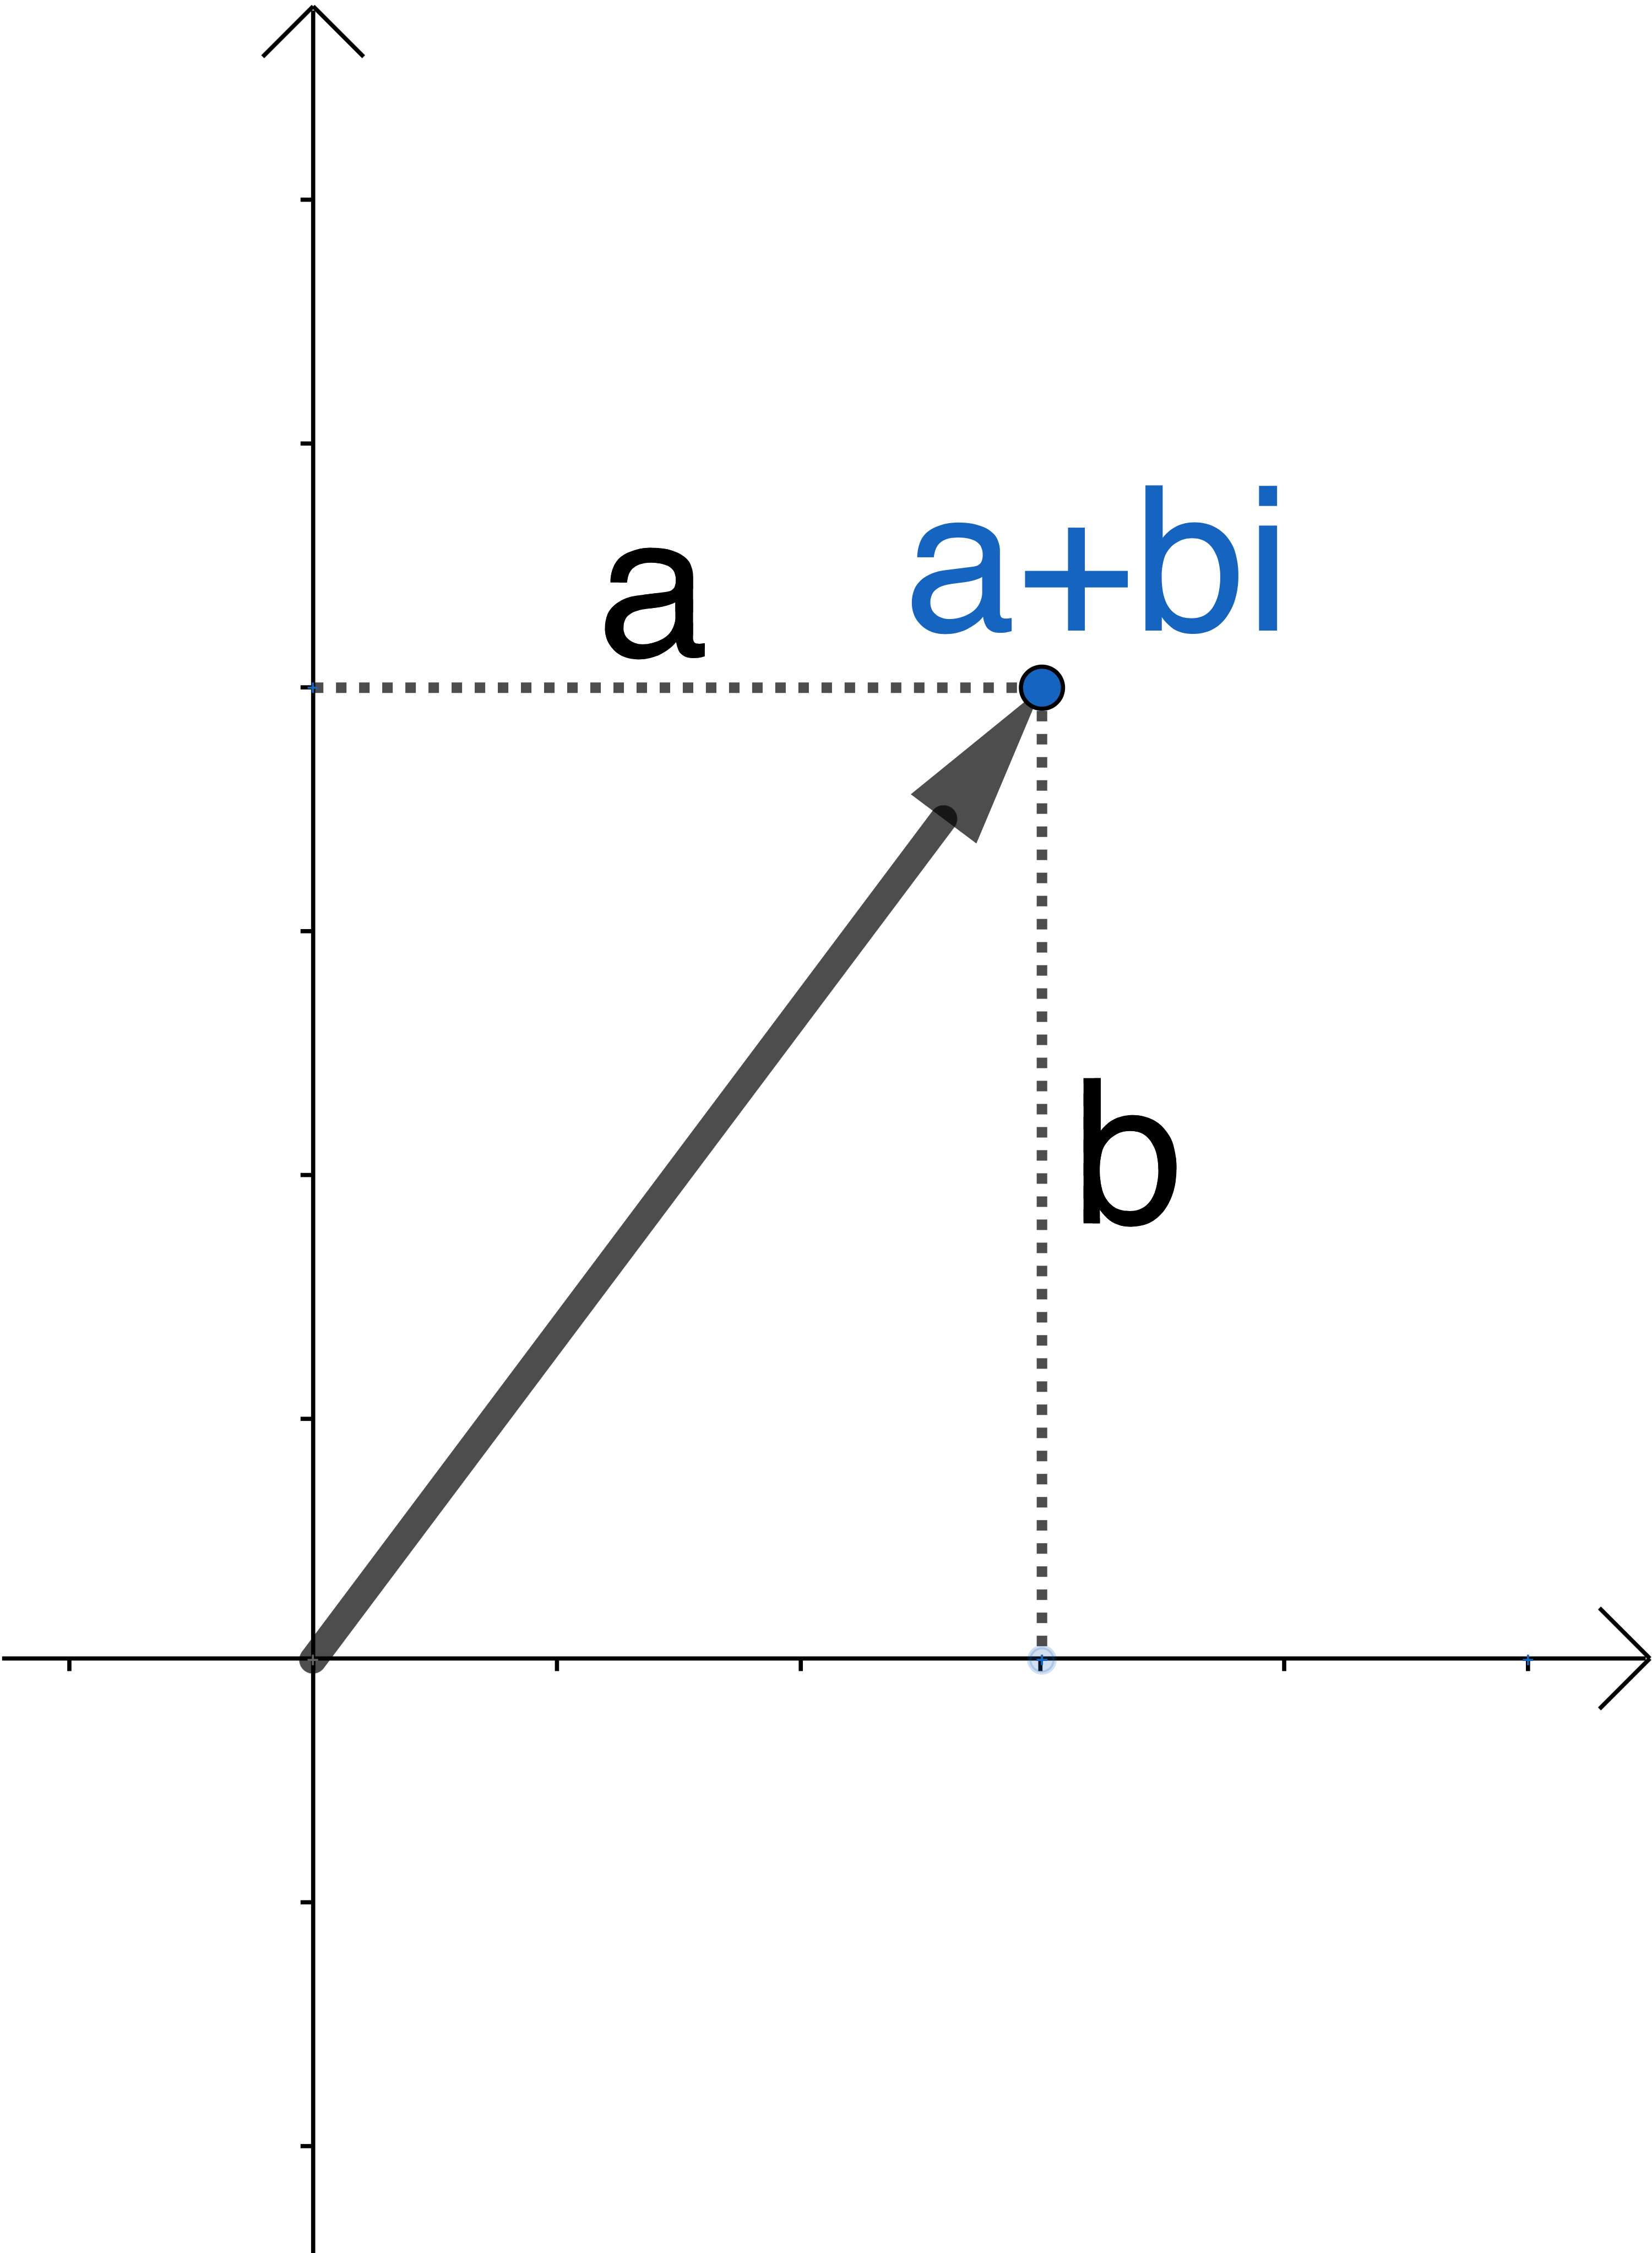
\includegraphics[scale=0.8]{complex-plane.png}
	\column{0.4\textwidth}
	We draw the complex number $z=a+bi$ as the point $(a, b)$ in $\mathbb{R}^2$.\vfill
	\begin{definition}
	The \emph{modulus of $z$} is its length in $\mathbb{R}^2$:
	\begin{equation*}
	|z| = \left| \left[
	\begin{array}{c}
	a\\
	b
	\end{array}
	\right]\right| = \sqrt{a^2+b^2}
	\end{equation*}
	\end{definition}
\end{columns}
\end{frame}

\begin{frame}{Addition of complex numbers}
\begin{columns}
\column{0.4\textwidth}
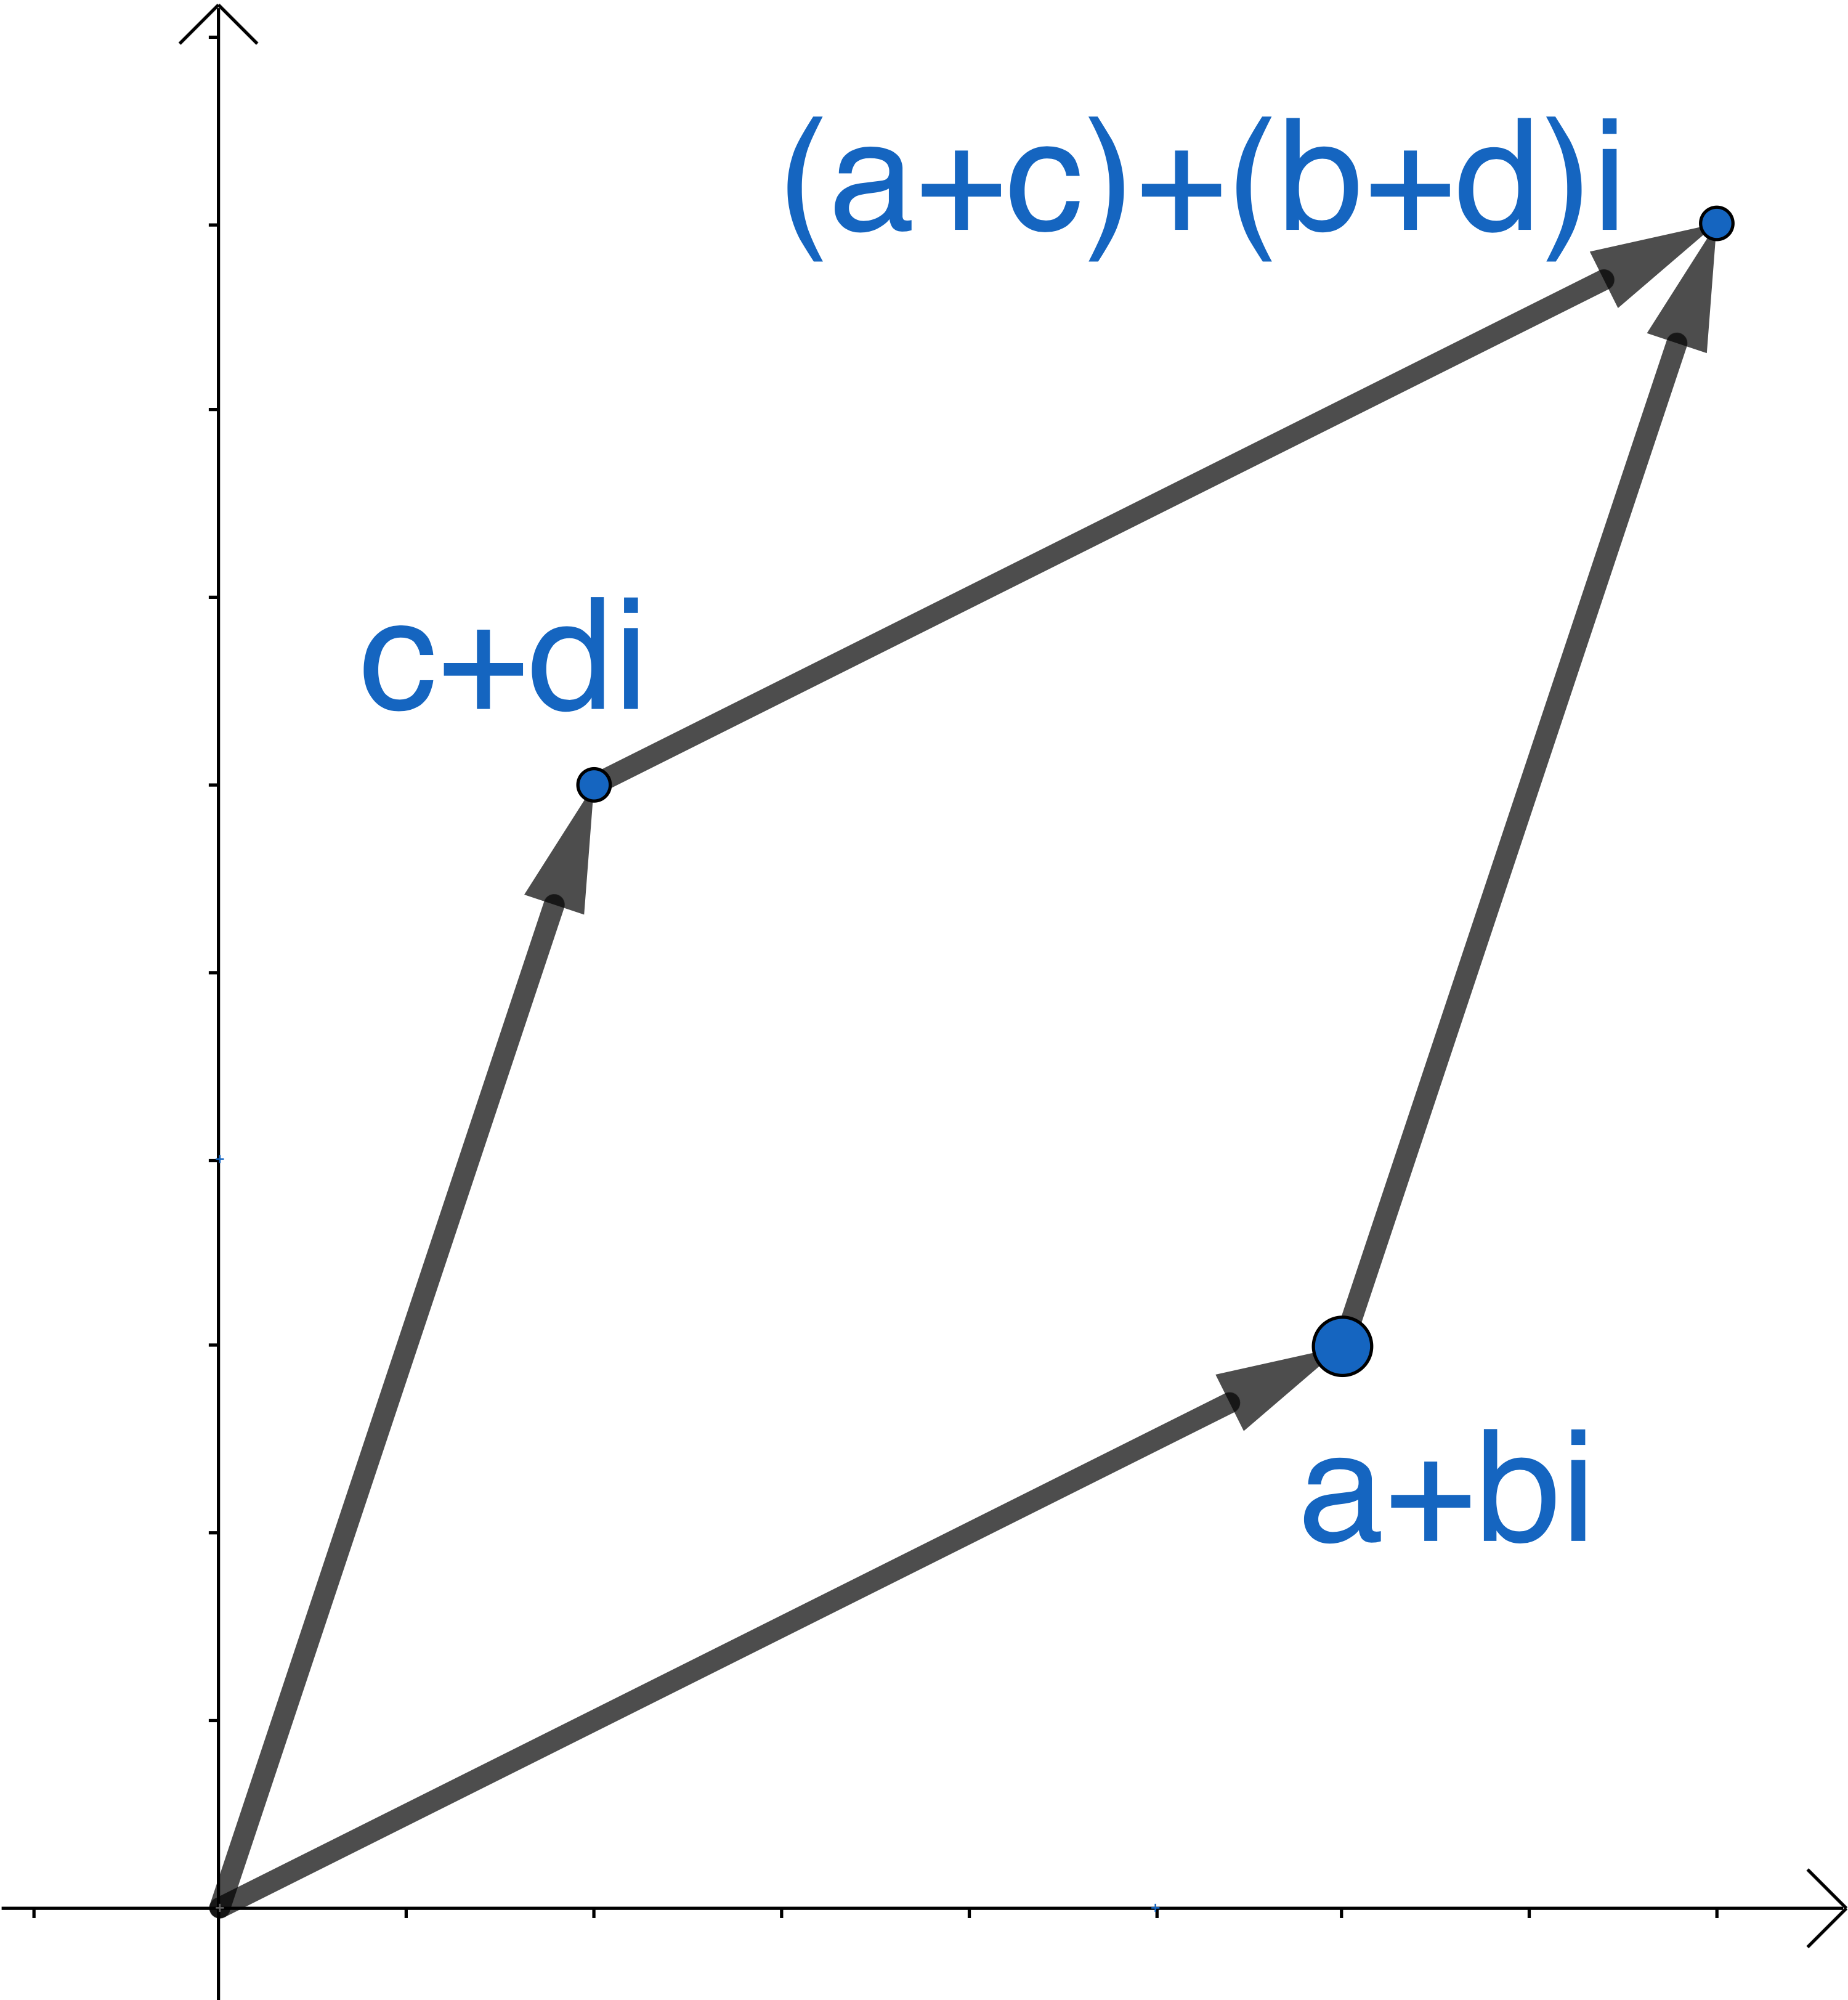
\includegraphics[scale=0.5]{complex-addition.png}
\column{0.5\textwidth}
Complex addition is defined component-wise:
\begin{equation*}
(a+ib)+(c+id) = (a+c)+(b+d)i
\end{equation*}
and therefore has the same graphical interpretation as the addition of vectors in $\mathbb{R}^2$.
\end{columns}
\end{frame}

\begin{frame}{Graphical interpretation of multiplication}
Next time.
\end{frame}

\begin{frame}{Conjugate}
\begin{columns}
	\column{0.5\textwidth}
	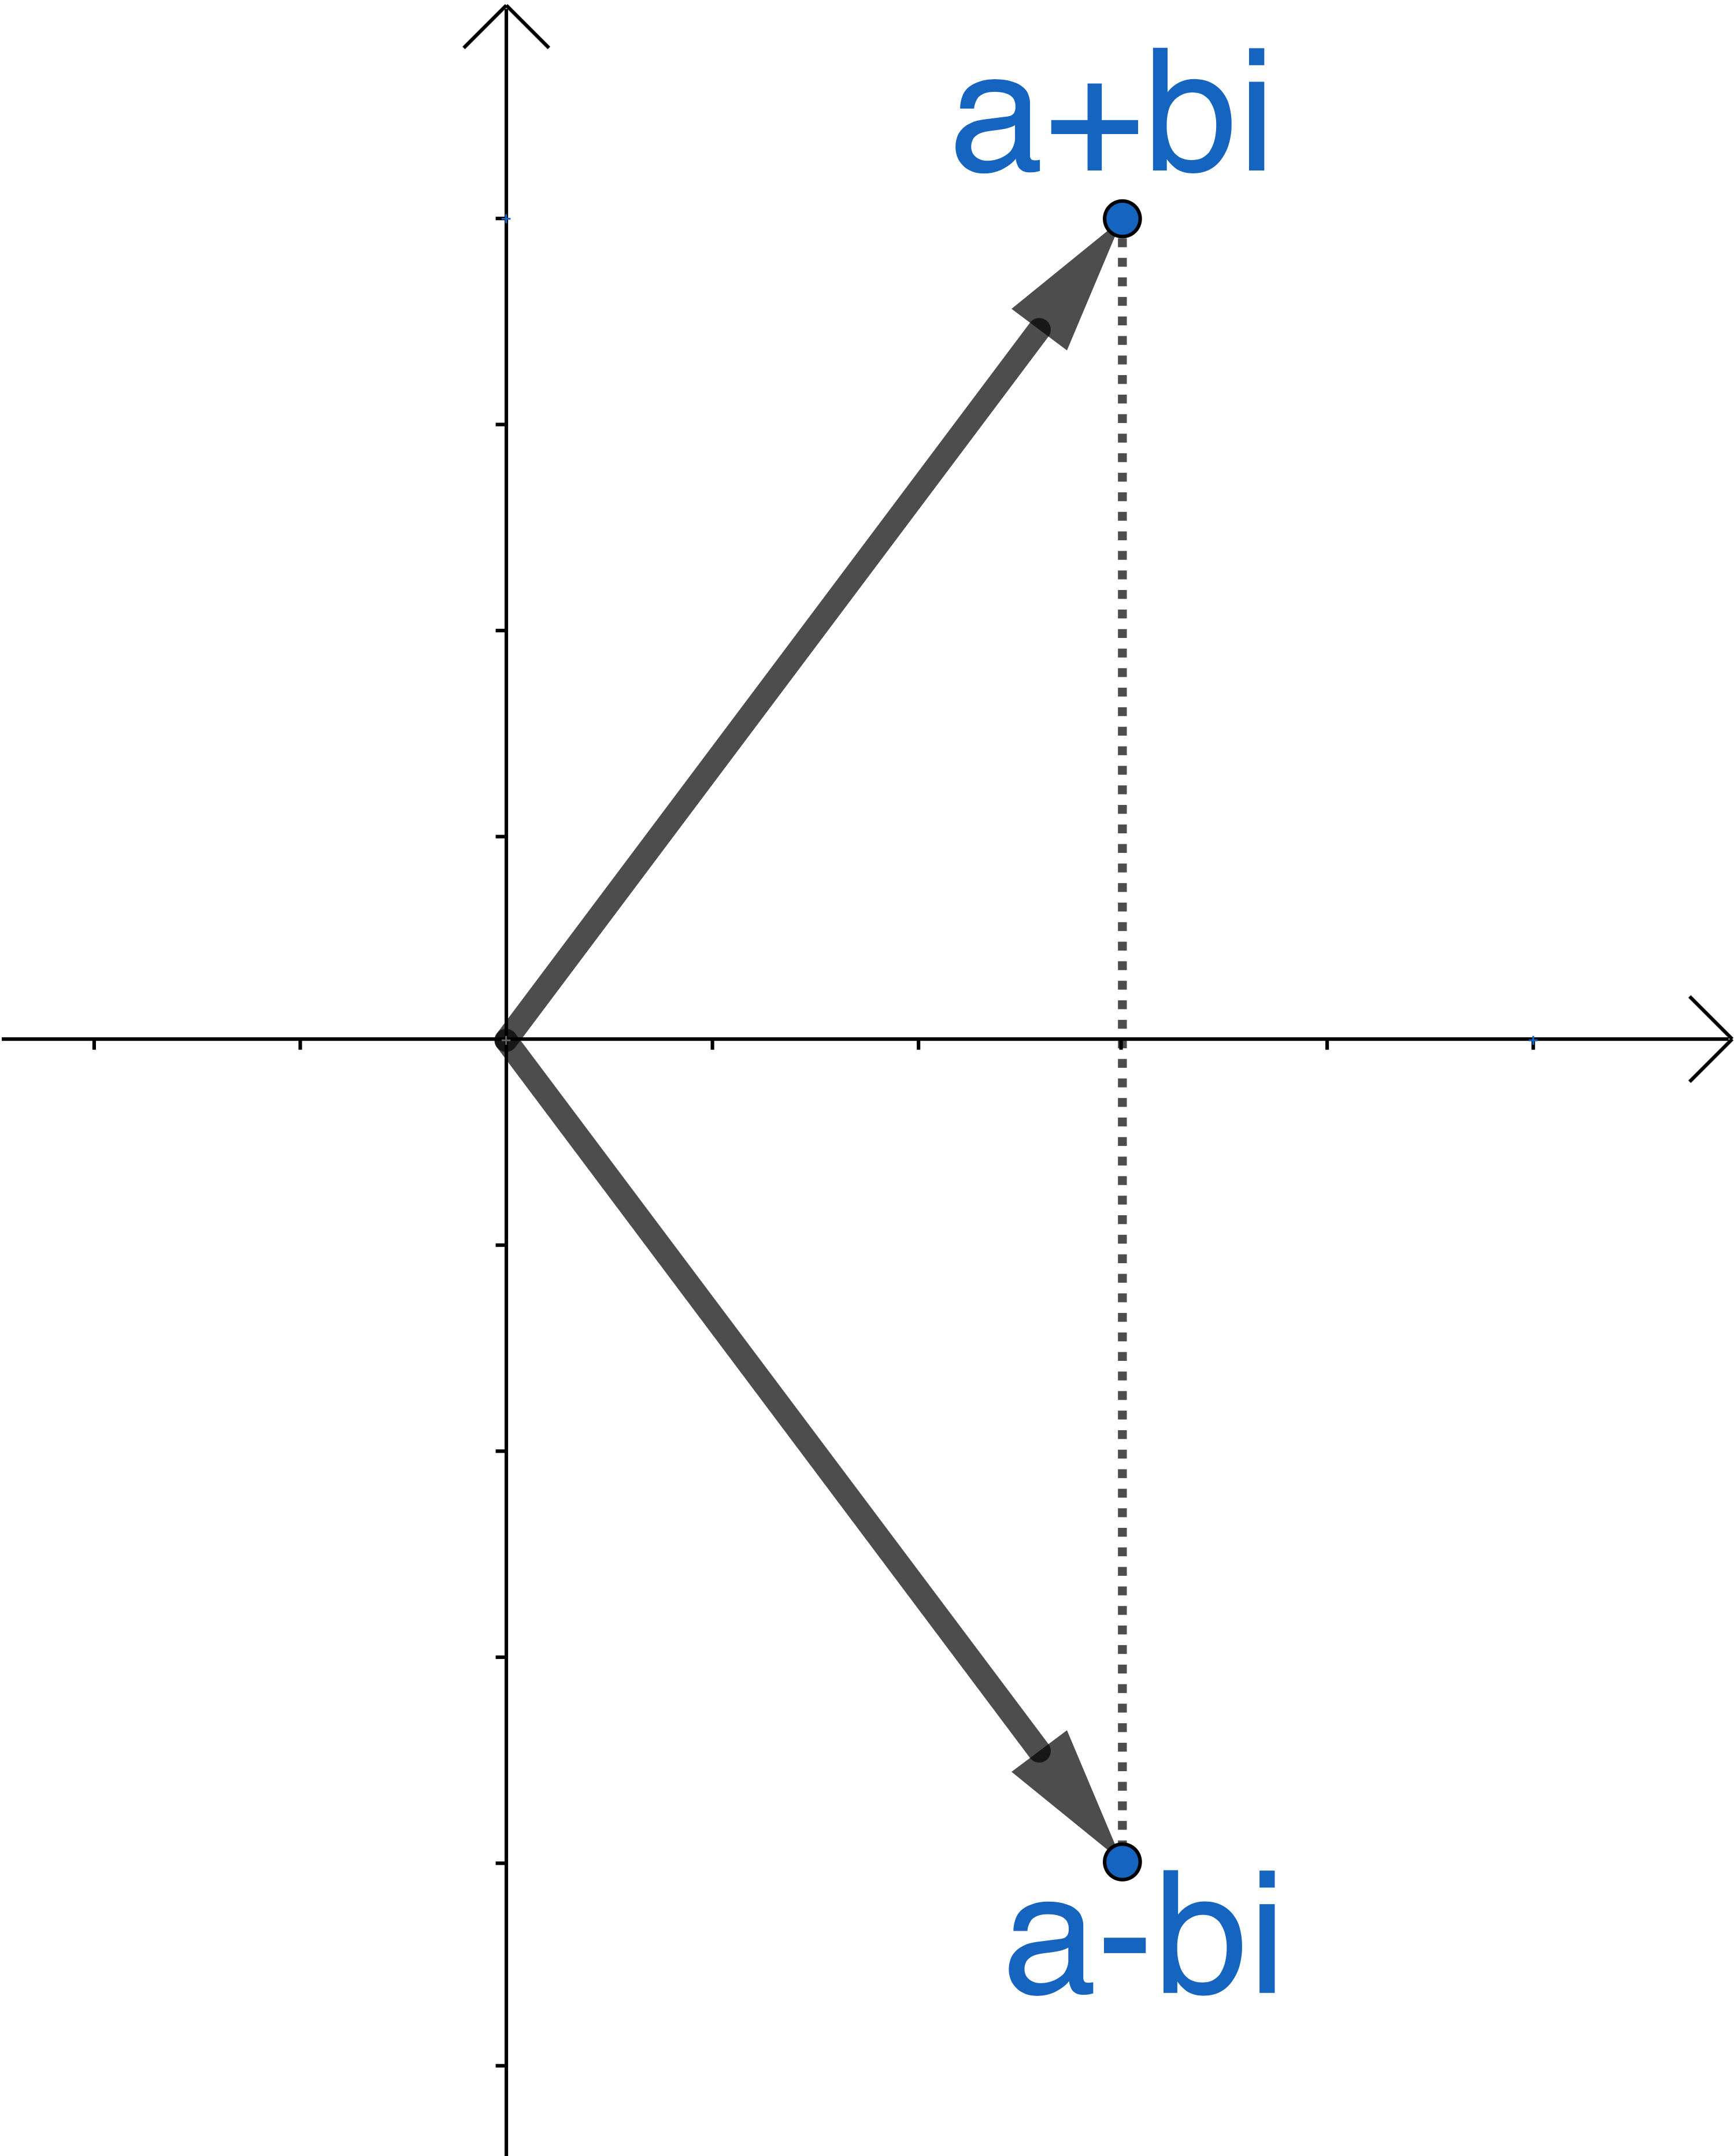
\includegraphics[scale=0.6]{conjugate.png}
	\column{0.4\textwidth}
	\begin{definition}[Conjugate]
	If
	\begin{equation*}
	z=a+bi
	\end{equation*}
	then
	\begin{equation*}
	\overline{z} = a-bi
	\end{equation*}
	\end{definition}
\end{columns}
\end{frame}

\begin{frame}{Properties of conjugate}
Let $z$ and $w$ be complex numbers.
\begin{itemize}
\item
$\overline{z\pm w} = \overline{z} \pm \overline{w}$.
\item
$\overline{(zw)} = \overline{z}~ \overline{w}$.
\item
$\overline{(\overline{z})}=z$.
\item
$\overline{\left(\frac{z}{w}\right)} =
\frac{\overline{z}}{\overline{w}}$.
\item
$z$ is real if and only if $\overline{z}=z$.
\end{itemize}
If $z=a+bi$, then
\[ z\overline{z}=
(a+bi)(a-bi)=
a^2 + b^2.\]
\end{frame}

\begin{frame}{Examples}
\begin{example}
	\begin{itemize}
		\item $|-3+4i|$
		% ANS: 5
		\item $|3-2i|$
		% ANS: sqrt(13)
		\item $|i|$
		% ANS: 1
	\end{itemize}
\end{example}
\begin{example}
\begin{itemize}
\item $\overline{3+4i}$
\item $\overline{-2+5i}$
\item $\overline{i}$
\item $\overline{7}$
\end{itemize}
\end{example}
\end{frame}


\end{document}